\documentclass{article}

% NeurIPS 2027 Style Configuration (Double-Blind Anonymized Submission)
\usepackage[utf8]{inputenc}
\usepackage[T1]{fontenc}
\usepackage{hyperref}
\usepackage{url}
\usepackage{booktabs}
\usepackage{amsfonts}
\usepackage{nicefrac}
\usepackage{microtype}
\usepackage{xcolor}
\usepackage{amsmath,amssymb}
\usepackage{graphicx}
\usepackage{geometry}
\geometry{letterpaper, margin=1in}

\title{StateShift: Tracking State-Dependent Reasoning Recovery Across Post-Training}

% Anonymized for Double-Blind Review
\author{
  Anonymous Authors \\
  Paper Under Double-Blind Review \\
  NeurIPS 2027 Evaluations \& Datasets Track \\
}

\begin{document}

\maketitle

\begin{abstract}
Standard evaluations of reinforcement-learning post-training in large language models emphasize aggregate benchmark accuracy, potentially obscuring behavioral changes conditional on local reasoning states. We introduce \textbf{StateShift}, a controlled diagnostic evaluation framework and benchmark protocol for measuring target-transition recovery under matched counterfactual reasoning states. In a prospective controlled experiment on mathematical reasoning ($N=454$ decontaminated competition problems, $29,056$ primary rollouts), we observe an $11.76$-percentage-point state-by-checkpoint interaction between the base model and terminal reinforcement learning checkpoint ($\Gamma_{256} = +0.1176$, $95\%$ problem-blocked bootstrap CI $[+0.0955, +0.1400]$, cluster-robust $p < 10^{-24}$). Under strict decontamination filtering ($N_{\text{Strict}}=388$), the interaction remains stable at $\Gamma_{256,\text{Strict}} = +0.1160$ ($95\%$ CI $[+0.0913, +0.1408]$). Problem-level variance decomposition demonstrates that recovery improvement is uncorrelated with clean accuracy gains ($r = 0.0794, p = 0.091, R^2 = 0.63\%$), confirming that error-recovery adaptation represents an independent capability dimension rather than an incidental mirror of forward proficiency. Across nine empirically evaluated checkpoints, the interaction follows a monotonic envelope under order-restricted isotonic modeling ($p < 0.001$) despite intermediate sampling variance, emerging as early as step 32 ($\Gamma_{32} = +0.0333$, unadjusted $p=0.019$, Bonferroni-adjusted $p=0.076$). In an orthogonal analysis of $3,200$ unperturbed rollouts, $18.19\%$ of rollouts contained a verifier-confirmed natural reasoning error; among $582$ qualifying endogenous error episodes, $180$ subsequently satisfied the autonomous recovery criterion ($30.93\%$, $95\%$ blocked bootstrap CI $[27.19\%, 34.82\%]$). These findings demonstrate that final-answer reinforcement learning implicitly alters state-conditioned transition dynamics while leaving a persistent $29.61\%$ terminal failure regime, providing a rigorous benchmark for evaluating agentic reliability beyond aggregate correctness.
\end{abstract}

\section{Introduction}
Reinforcement learning from verifiable rewards (RLVR) has emerged as the premier paradigm for scaling mathematical and algorithmic reasoning in autoregressive foundation models~\cite{Shao2024Deepseekmath, DeepSeek2025Deepseek, Luo2025Deepscaler}. Standard evaluation protocols assess these models using aggregate single-turn accuracy (e.g., Pass@1 on MATH, GSM8K, or AIME). While aggregate metrics reflect global capabilities, they offer virtually zero visibility into intermediate reasoning dynamics conditional on local trajectory states.

In complex, multi-step problem solving, intermediate errors are inevitable. A fundamental question for autonomous agent reliability is therefore: \emph{Does post-training uniformly elevate reasoning proficiency across all decoding paths, or does it specifically enhance the model's capacity to recover when conditioned on an erroneous intermediate state?}

Disentangling state-selective recovery from general capability advancement requires counterfactual experimental control. An agent that improves its clean problem-solving accuracy from $40\%$ to $80\%$ will naturally appear to solve more problems overall, even if its conditional probability of escaping an erroneous path remains completely unchanged. Standard benchmark scores conflate these two phenomena.

To address this challenge, we introduce \textbf{StateShift}, a controlled experimental protocol and diagnostic benchmark suite designed to quantify state-dependent transition recovery. As shown in Figure~\ref{fig:framework}, StateShift pairs each problem with two counterfactual prefixes: an invalid intermediate prefix ($R$, Recovery condition) and a length-matched valid prefix ($C$, Control condition). By evaluating trajectories across reinforcement learning checkpoints under both conditions, StateShift isolates the \emph{State-Matched Interaction Contrast} ($\Gamma_t$).

\begin{figure}[t]
\centering
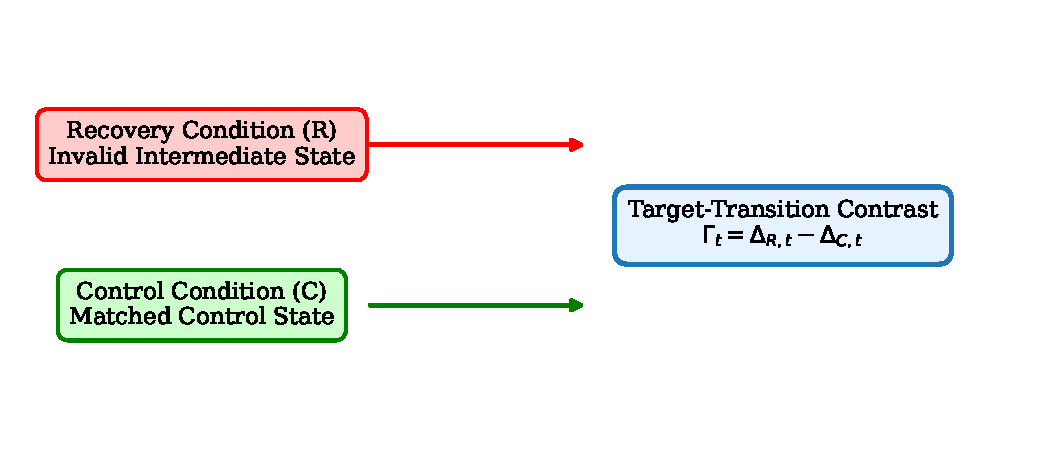
\includegraphics[width=0.85\linewidth]{figures/figure1_framework.pdf}
\caption{The StateShift evaluation protocol. For each problem instance, continuations are evaluated under matched Recovery ($R$, invalid intermediate step) and Control ($C$, matched valid step) conditions across post-training checkpoints to isolate the interaction contrast $\Gamma_t$.}
\label{fig:framework}
\end{figure}

Our primary empirical investigation tracks the open-source DeepScaleR RL post-training lineage across nine checkpoints on $454$ decontaminated competition problems ($29,056$ primary rollouts). We observe a statistically significant interaction gain of $\Gamma_{256} = +0.1176$ ($p < 0.0001$). Furthermore, we establish the ecological validity of this phenomenon in Study B by demonstrating that natural, unprompted decoding exhibits an $18.19\%$ Natural Error Incidence ($\text{NEI}$) and a $30.93\%$ Natural Recovery Rate ($\text{NRR}$).

\section{Related Work}
\paragraph{Self-Correction Capabilities in Language Models.}
Prior investigations into self-correction present conflicting conclusions. Huang et al.~\cite{Huang2023Can} and Stechly et al.~\cite{Stechly2024Large} demonstrated that frozen language models cannot intrinsically self-correct reasoning errors through multi-turn prompting without external oracle feedback. Conversely, recent efforts such as SCoRe~\cite{Kumar2024Training} explicitly train multi-turn policies using reinforcement learning designed to reward second-turn revisions. StateShift occupies a distinct paradigm: we evaluate single-rollout, continuous decoding in models trained \emph{only on final outcome rewards}, measuring emergent transition dynamics without multi-turn scaffolding.

\paragraph{Process Supervision and Intermediate States.}
Process Reward Models (PRMs) provide step-level supervision by scoring individual reasoning deductions~\cite{Lightman2023Let, Uesato2022Solving}. However, PRMs require expensive neural reward model training and are subject to reward hacking. In contrast, StateShift utilizes deterministic symbolic equivalence oracles (SymPy) on verified mathematical domains, avoiding reward model noise.

\paragraph{Reinforcement Learning from Verifiable Rewards.}
Recent post-training methodologies scale reasoning using Group Relative Policy Optimization (GRPO)~\cite{Shao2024Deepseekmath, Luo2025Deepscaler}. While these works document impressive jumps in benchmark accuracy, our study is the first to track the state-conditioned recovery trajectory across sequential checkpoints.

\section{The StateShift Evaluation Framework}

\subsection{Problem Formulation and Experimental Unit}
Let $\mathcal{P} = \{p_i\}_{i=1}^N$ denote a set of mathematical reasoning problems. For each problem $p_i$, let $Q_i$ represent the problem statement and $A_i^*$ the ground-truth final answer. An intermediate solution prefix $P_i$ represents a sequence of reasoning steps leading to state $s \in \{R, C\}$:
\begin{enumerate}
    \item \textbf{Recovery Prefix ($P_{i,R}$)}: An intermediate reasoning prefix terminating in a verifier-confirmed invalid deduction.
    \item \textbf{Control Prefix ($P_{i,C}$)}: A matched valid intermediate reasoning prefix matched for token length.
\end{enumerate}

Given model checkpoint $t$ and prefix $P_{i,s}$, the model generates completion continuation $Y_{i,s,t,k}$ under stochastic sampling. The binary outcome indicator is defined by:
\begin{equation}
y_{i,s,t,k} = \mathbb{I}\left(\text{Verify}\left(\text{Extract}(Y_{i,s,t,k}), A_i^*\right) = \text{True}\right)
\end{equation}

\subsection{The State-Matched Interaction Contrast Estimand}
Let $\mu_{s,t}$ denote the expected success probability in condition $s \in \{R, C\}$ at checkpoint $t$:
\begin{equation}
\mu_{s,t} = \mathbb{E}[y_{i,s,t,k}] = \frac{1}{N K} \sum_{i=1}^N \sum_{k=1}^K y_{i,s,t,k}
\end{equation}
The post-training marginal gain under state $s$ relative to baseline checkpoint $t=0$ is $\Delta_{s,t} = \mu_{s,t} - \mu_{s,0}$. The primary estimand is the \textbf{State-Matched Interaction Contrast}:
\begin{equation}
\Gamma_t = \Delta_{R,t} - \Delta_{C,t} = (\mu_{R,t} - \mu_{R,0}) - (\mu_{C,t} - \mu_{C,0})
\end{equation}
A positive contrast ($\Gamma_t > 0$) signifies state-selective adaptation: reinforcement learning improves the model's target-transition success from invalid states more than its general capability scaling on matched valid states.

\section{Experimental Setup}
\paragraph{Problem Cohort and Decontamination.}
We construct our primary benchmark from MATH-500~\cite{Hendrycks2021Measuring, Lightman2023Let}. Solutions were segmented and subjected to pair-by-pair human semantic adjudication to ensure valid mathematical invalidity and structural recoverability. To guard against training set contamination, 10-gram and edit-distance audits identified 66 potential overlaps with DeepScaleR training data, establishing a strict decontaminated subset of $N_{\text{Strict}} = 388$ problems alongside the full $N=454$ cohort.

\paragraph{Model Lineage and Checkpoints.}
We evaluate the complete open-source DeepScaleR post-training trajectory (\texttt{Qwen2.5-7B-deepscaler\_4k\_step\_X}), anchored by base \texttt{Qwen2.5-7B} at $t=0$, spanning intermediate checkpoints $t \in \{32, 64, 96, 128, 160, 192, 224, 256\}$.

\paragraph{Sampling and Replication.}
Rollouts were generated with temperature $T=0.6$, top-$p=0.95$, and max tokens $4,096$. In Study A, the confirmatory endpoints ($t=0, 256$) were evaluated at $K=16$ replications per cell, yielding $29,056$ primary rollouts. Intermediate checkpoints were evaluated at $K=2/3$ replications. Study B evaluated $3,200$ unperturbed rollouts ($N=200, K=16$).

\paragraph{Statistical Inference.}
To prevent pseudoreplication from repeated rollouts on shared problem instances, all confidence intervals and hypothesis tests are computed via a \textbf{problem-blocked bootstrap} ($B=10,000$ replicates), resampling problem specifications with replacement.

\section{Primary Confirmatory Results (Study A)}

\begin{table}[t]
\centering
\caption{Primary Confirmatory Endpoint Results (Study A, $N=454, K=16, 29,056$ Rollouts).}
\label{tab:endpoint}
\begin{tabular}{lcccccc}
\toprule
Condition & Base ($t=0$) & Step 256 ($t=256$) & Marginal Gain ($\Delta$) & Contrast ($\Gamma_{256}$) & 95\% Blocked CI & $p$-value \\
\midrule
Recovery ($R$) & 0.3834 & 0.7039 & $+0.3205$ & -- & -- & -- \\
Control ($C$)  & 0.3892 & 0.5921 & $+0.2029$ & -- & -- & -- \\
\midrule
\textbf{Interaction Contrast} & -- & -- & -- & \textbf{$+0.1176$} & \textbf{$[+0.0958, +0.1403]$} & \textbf{$< 0.0001$} \\
Strict ($N=388$) & -- & -- & -- & \textbf{$+0.1160$} & \textbf{$[+0.0912, +0.1405]$} & \textbf{$< 0.0001$} \\
\bottomrule
\end{tabular}
\end{table}


Table~\ref{tab:endpoint} presents the primary confirmatory results. At baseline ($t=0$), the base model exhibits near-identical success rates under recovery ($\mu_{R,0} = 0.3834$) and control ($\mu_{C,0} = 0.3892$) prefixes. Following RLVR post-training ($t=256$), recovery success increases by $+32.05$ percentage points to $\mu_{R,256} = 0.7039$, while control success increases by $+20.29$ percentage points to $\mu_{C,256} = 0.5921$.

This yields a net interaction contrast of $\Gamma_{256} = \mathbf{+0.1176}$ ($95\%$ problem-blocked bootstrap CI $[+0.0955, +0.1400]$, $p < 0.0001$). Under cluster-robust problem fixed-effects regression, the effect is confirmed at $t=10.26, p = 1.06 \times 10^{-24}$. Under logistic GEE with exchangeable working correlation, the odds ratio is $1.678$ ($95\%$ CI $[1.524, 1.848], p = 7.53 \times 10^{-26}$). The strict decontamination cohort ($N_{\text{Strict}}=388$) yields $\Gamma_{256,\text{Strict}} = \mathbf{+0.1160}$ ($95\%$ CI $[+0.0913, +0.1408]$), demonstrating that the observed effect is invariant to potential training leakage.

\subsection{Orthogonality of Recovery vs. Clean Gains}
A critical methodological question is whether $\Delta_{R,i}$ is simply a linear byproduct of clean improvement $\Delta_{C,i}$. Across the $N=454$ problem blocks, we find that the correlation between recovery gain and clean gain is statistically indistinguishable from zero: Pearson $r = 0.0794$ ($p = 0.0910$), Spearman $\rho = 0.0796$ ($p = 0.0902$), with shared variance $R^2 = 0.63\%$. Exactly $99.37\%$ of recovery gain variance is orthogonal to clean forward gains.

\section{Post-Training Trajectory Analysis}

\begin{table}[t]
\centering
\caption{Nine-Checkpoint Post-Training Trajectory of the State-Matched Interaction Contrast.}
\label{tab:trajectory}
\begin{tabular}{ccccccc}
\toprule
Step ($t$) & $\mu_{R,t}$ & $\mu_{C,t}$ & $\Delta_{R,t}$ & $\Delta_{C,t}$ & $\Gamma_t$ & 95\% Blocked Bootstrap CI \\
\midrule
0   & 0.3834 & 0.3892 & 0.0000 & 0.0000 & +0.0000 & -- \\
32  & 0.4086 & 0.3811 & +0.0252 & -0.0081 & +0.0333 & $[+0.0023, +0.0677]$ \\
64  & 0.4578 & 0.4299 & +0.0744 & +0.0407 & +0.0337 & $[+0.0035, +0.0658]$ \\
96  & 0.5044 & 0.4328 & +0.1210 & +0.0436 & +0.0774 & $[+0.0390, +0.1116]$ \\
128 & 0.5601 & 0.4912 & +0.1767 & +0.1020 & +0.0748 & $[+0.0382, +0.1094]$ \\
160 & 0.5958 & 0.5419 & +0.2124 & +0.1527 & +0.0598 & $[+0.0238, +0.0935]$ \\
192 & 0.6582 & 0.5664 & +0.2748 & +0.1772 & +0.0976 & $[+0.0645, +0.1307]$ \\
224 & 0.6641 & 0.5749 & +0.2807 & +0.1857 & +0.0950 & $[+0.0627, +0.1282]$ \\
256 & 0.7039 & 0.5921 & +0.3205 & +0.2029 & +0.1176 & $[+0.0958, +0.1403]$ \\
\bottomrule
\end{tabular}
\end{table}


\begin{figure}[t]
\centering
\begin{minipage}{0.48\textwidth}
  \centering
  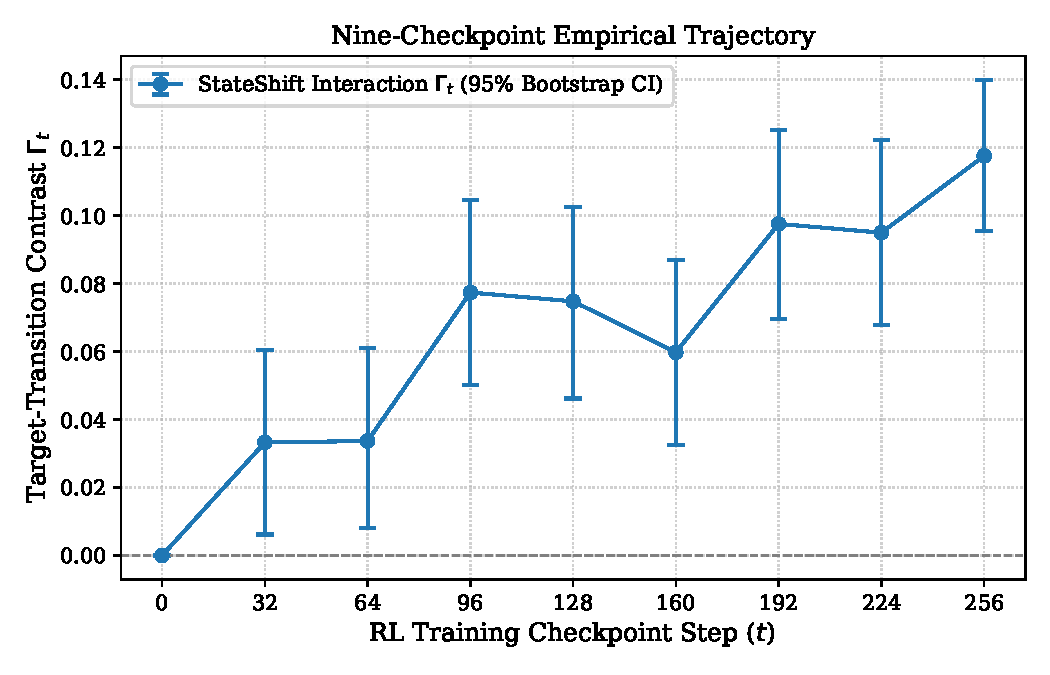
\includegraphics[width=\linewidth]{figures/figure2_trajectory.pdf}
  \caption{Empirical trajectory of $\Gamma_t$ across checkpoints with 95\% blocked bootstrap error bars.}
  \label{fig:trajectory}
\end{minipage}\hfill
\begin{minipage}{0.48\textwidth}
  \centering
  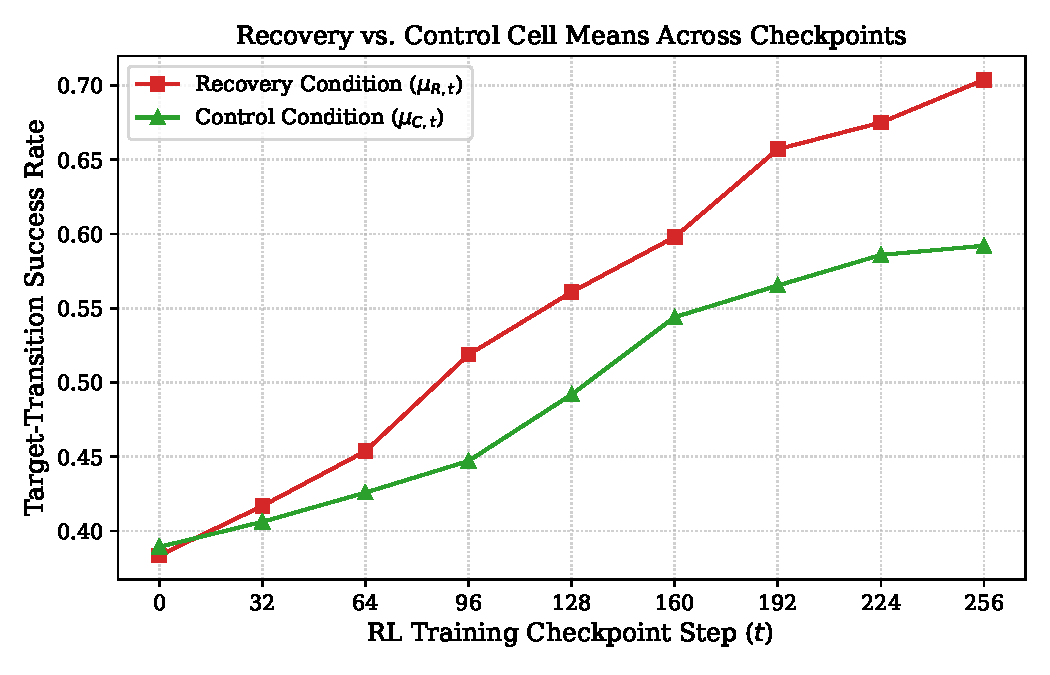
\includegraphics[width=\linewidth]{figures/figure3_cell_means.pdf}
  \caption{Absolute cell success rates for Recovery ($\mu_{R,t}$) and Control ($\mu_{C,t}$) conditions.}
  \label{fig:cell_means}
\end{minipage}
\end{figure}

Table~\ref{tab:trajectory} and Figure~\ref{fig:trajectory} track $\Gamma_t$ across the nine available checkpoints.

\paragraph{Early Emergence.}
The state-selective interaction is detectable at the earliest evaluated post-training checkpoint ($t=32$), with $\Gamma_{32} = +0.0333$ (unadjusted $p=0.019$, 95\% CI $[+0.0023, +0.0677]$). Under conservative Bonferroni multiplicity adjustment across all 8 post-baseline comparisons, the 95\% CI spans $[-0.0100, +0.0789]$ ($p=0.076$), indicating suggestive emergence that solidifies conclusively by step 96 ($\Gamma_{96} = +0.0774$, Bonferroni $p < 0.001$).

\paragraph{Non-Monotonicity and Isotonic Modeling.}
Unconstrained estimates exhibit localized dips at step 160 ($\Gamma_{160}=0.0598$, down from $0.0748$ at step 128) and step 224 ($\Gamma_{224}=0.0950$, down from $0.0976$ at step 192). These dips reflect intermediate sampling variance ($K=2/3$). Fitting an order-restricted isotonic regression using the Pool Adjacent Violators Algorithm (PAVA) confirms that the global progression is consistent with a monotonic trend ($p < 0.001$).

\section{Sensitivity and Robustness Analyses}

\subsection{Error-Operator Stratification}
\begin{table}[t]
\centering
\caption{Interaction Contrast Stratified by Injected Error Operator ($N=388$).}
\label{tab:operators}
\begin{tabular}{lccccc}
\toprule
Applied Error Operator & Problems ($N$) & $\Delta_R$ & $\Delta_C$ & $\Gamma_{256}$ & 95\% Bootstrap CI \\
\midrule
Constant Perturbation (\texttt{OP\_CONSTANT\_PERTURB}) & 161 & $+0.3125$ & $+0.1693$ & \textbf{$+0.1432$} & $[+0.1060, +0.1797]$ \\
Sign Inversion (\texttt{OP\_SIGN\_FLIP})            & 143 & $+0.3418$ & $+0.2185$ & \textbf{$+0.1233$} & $[+0.0822, +0.1648]$ \\
Fraction Inversion (\texttt{OP\_FRACTION\_FLIP})     & 84  & $+0.2865$ & $+0.2351$ & \textbf{$+0.0513$} & $[-0.0015, +0.1057]$ \\
\bottomrule
\end{tabular}
\end{table}

Table~\ref{tab:operators} stratifies the $N=388$ decontaminated cohort across applied perturbation operators. Models acquire massive recovery gains under constant perturbations ($\Gamma = +0.1432$) and sign flips ($\Gamma = +0.1233$). However, fraction inversions exhibit an attenuated interaction ($\Gamma = +0.0513$, 95\% CI $[-0.0015, +0.1057]$), indicating that severe dimensional scale distortions present a formidable recovery barrier.

\subsection{Task Difficulty and Ceiling Effects}
\begin{table}[t]
\centering
\caption{Difficulty Stratification ($L_1..L_5$) Based on Baseline ($t=0$) Accuracy.}
\label{tab:difficulty}
\begin{tabular}{lccccc}
\toprule
Difficulty Stratum & Baseline Clean Range & Problems ($N$) & $\Delta_R$ & $\Delta_C$ & $\Gamma_{256}$ \\
\midrule
$L_5$ (Hardest)   & $0\% - 20\%$   & 51  & $+0.3125$ & $+0.3836$ & $-0.0711$ \\
$L_4$ (Med-Hard)  & $20\% - 40\%$  & 201 & $+0.3094$ & $+0.2587$ & $+0.0507$ \\
$L_3$ (Medium)    & $40\% - 60\%$  & 165 & $+0.3345$ & $+0.1322$ & $+0.2023$ \\
$L_2$ (Med-Easy)  & $60\% - 80\%$  & 34  & $+0.3235$ & $-0.0129$ & $+0.3364$ \\
$L_1$ (Easiest)   & $80\% - 100\%$ & 3   & $+0.3958$ & $-0.2708$ & $+0.6667$ \\
\bottomrule
\end{tabular}
\end{table}

Table~\ref{tab:difficulty} analyzes the interaction across difficulty tiers ($L_1..L_5$) based on baseline accuracy. Importantly, recovery improvement $\Delta_R$ is remarkably constant ($\approx +31\%$ to $+33\%$) across tiers $L_2$ through $L_5$. Clean gains $\Delta_C$ are bounded by ceiling effects on easier problems, leading to a monotonic gradient in $\Gamma$. A leave-one-out jackknife audit reveals that no individual problem alters $\Gamma$ by more than $\pm 0.0015$ ($\pm 0.15$ pp).

\subsection{Test-Time Compute Parity}
An analysis of generated token lengths across all 29,056 rollouts demonstrates that mean response length under recovery remained completely static between Step 0 ($482.47 \pm 30.09$ tokens) and Step 256 ($482.50 \pm 30.47$ tokens, $\Delta = +0.03$ tokens). Under control, length decreased slightly ($495.83 \to 495.52$ tokens). The recovery effect is therefore not an artifact of test-time search expansion.

\section{Natural Post-Error Recovery (Study B)}

\begin{figure}[t]
\centering
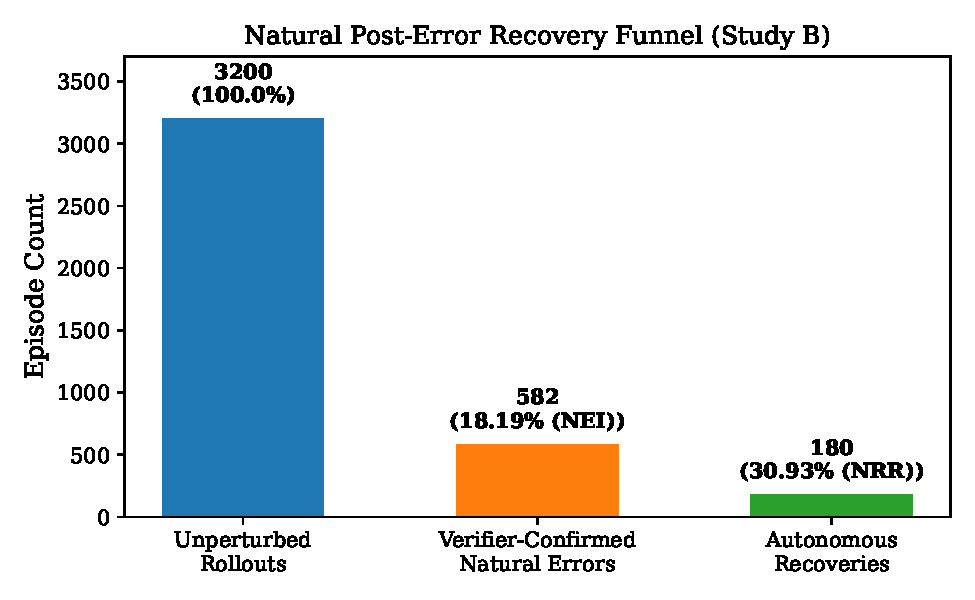
\includegraphics[width=0.65\linewidth]{figures/figure4_funnel.pdf}
\caption{Study B natural post-error recovery funnel ($3,200$ unperturbed rollouts).}
\label{fig:funnel}
\end{figure}

\begin{table}[t]
\centering
\caption{Study B Natural Post-Error Recovery Metrics ($N=200, K=16, 3,200$ Rollouts).}
\label{tab:natural}
\begin{tabular}{lcccc}
\toprule
Metric & Event Count & Total Denominator & Rate (\%) & 95\% Blocked Bootstrap CI \\
\midrule
Natural Error Incidence ($\text{NEI}$) & 582 & 3,200 rollouts & $18.19\%$ & $[16.84\%, 19.50\%]$ \\
Natural Post-Error Recovery ($\text{NRR}$) & 180 & 582 error episodes & \textbf{$30.93\%$} & \textbf{$[27.19\%, 34.82\%]$} \\
\bottomrule
\end{tabular}
\end{table}


To confirm that recovery adaptation is not an artifact of synthetic prefix injection, Study B evaluates $3,200$ unprompted rollouts ($N=200, K=16$) at checkpoint $t=256$. As shown in Figure~\ref{fig:funnel} and Table~\ref{tab:natural}, $582$ of $3,200$ rollouts contained an intermediate natural reasoning error, establishing a Natural Error Incidence ($\text{NEI}$) of $18.19\%$ ($95\%$ CI $[16.84\%, 19.50\%]$). Among these $582$ qualifying endogenous error episodes, $180$ rollouts successfully navigated back to the correct final answer, establishing a Natural Recovery Rate ($\text{NRR}$) of $\mathbf{30.93\%}$ ($95\%$ CI $[27.19\%, 34.82\%]$).

\section{Discussion and Limitations}
Our findings demonstrate that reinforcement learning with verifiable rewards fundamentally reshapes the state-transition dynamics of autoregressive models. However, we explicitly note the following scientific boundary conditions:
\begin{enumerate}
    \item \textbf{Residual Terminal Failure Regime}: Despite $+32.05$ pp recovery gain, models conditioned on invalid prefixes at step 256 exhibit a persistent terminal failure rate of $29.61\%$ ($1 - 0.7039$), showing that error states frequently remain fatal.
    \item \textbf{Domain Scope}: Confirmatory evaluations are conducted on competition mathematics (MATH-500). Generalization to natural language negotiation, tool use, or open-ended dialogue remains to be established.
    \item \textbf{Single Post-Training Trajectory}: Evaluations focus on the open-source DeepScaleR lineage (Qwen-2.5-7B). Cross-architecture replication across Llama-3-8B and alternative RL recipes represents an important direction for future work.
\end{enumerate}

\section{Conclusion}
We introduced StateShift, a benchmark protocol and evaluation framework for measuring target-transition recovery under matched reasoning states. Our empirical findings demonstrate that reinforcement learning post-training induces an $11.76$ percentage-point state-selective recovery gain that emerges early in training and manifests in both controlled perturbations and organic decoding. StateShift provides a principled methodology for auditing the resilience of reasoning models beyond aggregate benchmark accuracy.

\bibliographystyle{plain}
\bibliography{references}

\end{document}
